\documentclass{article}
\setlength\parindent{24pt}
\usepackage[margin=0.6in]{geometry}
\usepackage{indentfirst}
\usepackage{amsmath}
\usepackage{graphicx}
\usepackage{float}
\usepackage[utf8]{inputenc}
\usepackage{listings}
\usepackage{color}
\usepackage{enumerate}
\usepackage[portuguese]{babel}

\definecolor{dkgreen}{rgb}{0,0.6,0}
\definecolor{gray}{rgb}{0.5,0.5,0.5}
\definecolor{mauve}{rgb}{0.58,0,0.82}

\lstset{frame=tb,
  language=Matlab,
  aboveskip=3mm,
  belowskip=3mm,
  showstringspaces=false,
  columns=flexible,
  basicstyle={\small\ttfamily},
  numbers=none,
  numberstyle=\tiny\color{gray},
  keywordstyle=\color{blue},
  commentstyle=\color{dkgreen},
  stringstyle=\color{mauve},
  breaklines=true,
  breakatwhitespace=true,
  tabsize=4
}

\renewcommand{\baselinestretch}{1.0}

\begin{document}

\title{EA614 - Análise de Sinais \\
\large{EFC4 - Filtros Analógicos}}
\author{Rafael Gonçalves (186062)}
\date{\today}

\maketitle

\section{Filtro de Chebyshev}

\begin{enumerate}[(a)]
\item
    Segue o gráfico de $|H(j\omega)| \times \omega$:
 \begin{figure}[H]
 \centering
 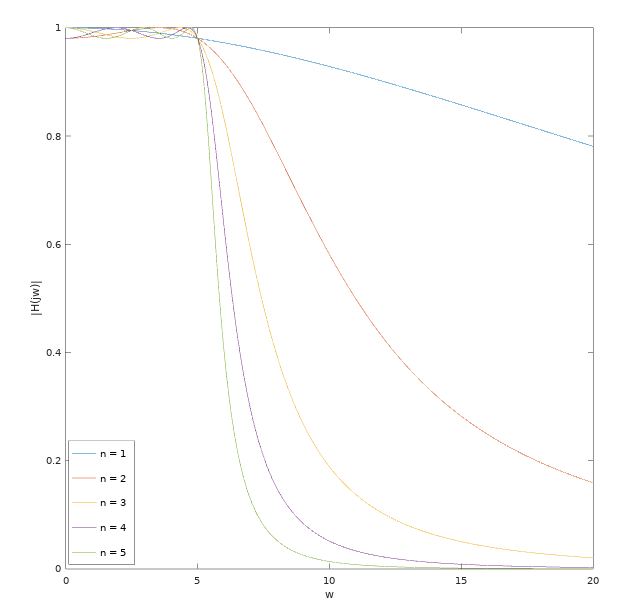
\includegraphics[width=0.5\textwidth]{images/hc_n.png}
     \caption{Módulo da resposta em frequência em função de $\omega$ para diferentes $n$}
 \end{figure}

        Percebe-se que o aumento do parâmetro $n$ promove uma diminuição mais abrupta do ganho após o ponto $\omega = \omega_C$. Por outro lado para $\omega < \omega_C$ o sinal apresenta mais oscilações conforme o aumento do parâmetro $n$. Nota-se que num ponto próximo ao ponto $\omega = \omega_C$ o valor do gráfico é o mesmo para essa configuração independente de $\epsilon$.

\break\vfill

\item
    Gráfico de $|H(j\omega)| \times \omega$:
 \begin{figure}[H]
 \centering
 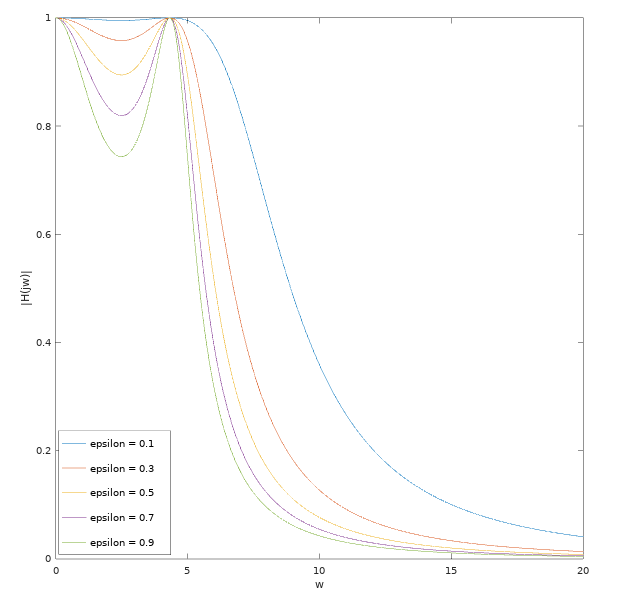
\includegraphics[width=0.5\textwidth]{images/hc_epsilon.png}
     \caption{Módulo da resposta em frequência em função de $\omega$ para diferentes $\epsilon$}
 \end{figure}

        É possível observar que o aumento parâmetro $\epsilon$ é responsável pelo aumento da amplitude das oscilações para $\omega < \omega_C$ bem como pela diminuição mais abrupta do ganho após o ponto $\omega  = \omega_C$. Num ponto próximo ao ponto $\omega = \omega_C$ o valor do gráfico para um mesmo $n$ coincide independente de $\epsilon$.

\break\vfill

\section{Filtro de Butterworth}

\item
    Gráfico de $|H(j\omega)| \times \omega$:
 \begin{figure}[H]
 \centering
 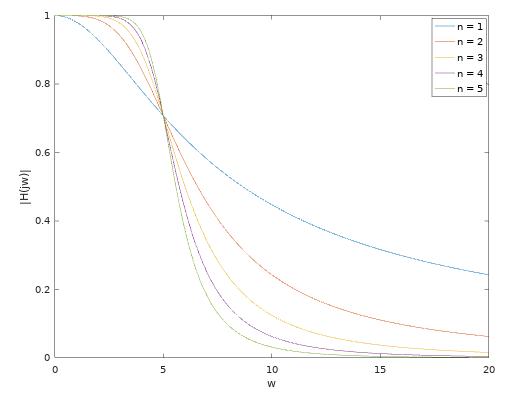
\includegraphics[width=0.5\textwidth]{images/hb_n.png}
     \caption{Módulo da resposta em frequência em função de $\omega$ para diferentes $n$}
 \end{figure}

        Observa-se que conforme o parâmetro $n$ aumenta, a curva começa a decair mais próximo ao ponto $\omega = \omega_C$, e também decai mais abruptamente (dando impressão de que a curva está mais "achatada" em torno do ponto $\omega = \omega_C$). Neste gráfico um fenômeno semelhante aos anteriores pode ser observado em que no ponto $\omega = \omega_C$ é o mesmo independente de $n$.

\break\vfill

\section{Filtragem de Pulso Retangular}

\item

    Modelando o pulso retangular como:

    \begin{equation}
        x(t) = u(t + \frac{\tau}{2}) - u(t - \frac{\tau}{2})
    \end{equation}

    Temos que sua transformada de Fourier é dada por:

    \begin{equation}
        X(j\omega) = \int \limits_{\frac{-\tau}{2}}^{\frac{\tau}{2}} x(t) e^{-j\omega t} dt
    \end{equation}

    \begin{equation}
        X(j\omega) = \int \limits_{\frac{-\tau}{2}}^{\frac{\tau}{2}} 1 \cdot e^{-j\omega t} dt
    \end{equation}

    \begin{equation}
        X(j\omega) = \left [ \frac{e^{-j\omega t}}{-j\omega} \right ] _{\frac{-\tau}{2}} ^{\frac{\tau}{2}} = \frac{e^{\frac{-j\omega\tau}{2}}}{-j\omega} - \frac{e^{\frac{j\omega\tau}{2}}}{-j\omega} = \frac{2}{\omega} \left [\frac{e^{\frac{j\omega\tau}{2}} - e^{\frac{-j\omega\tau}{2}}}{2j} \right ] = \frac{2}{\omega}sen(\frac{\tau\omega}{2})
    \end{equation}

Dado que $\tau = \frac{2\pi}{\omega_C}$:

\[
    \boxed{X(j\omega) = \frac{2}{\omega}sen(\frac{\pi\omega}{\omega_C})}
\]

    Gráfico de $|X(j\omega)| \times \omega$:

 \begin{figure}[H]
 \centering
 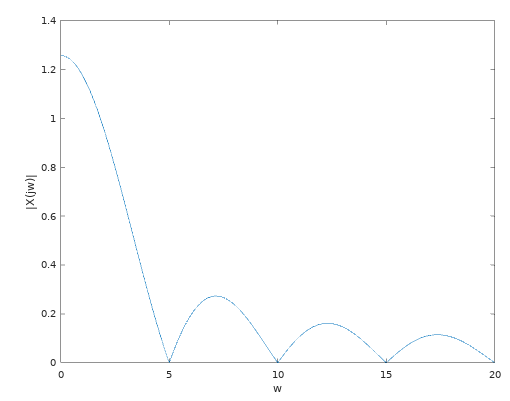
\includegraphics[width=0.5\textwidth]{images/Xjw.png}
     \caption{Módulo de $X(j\omega)$}
 \end{figure}

 Os pontos em que o valor de $|X(j\omega)|$ é zero são os pontos em que $\omega$ é múltiplo de $\omega_C$. Isso se dá pois nesta circunstância o argumento do seno em $X(j\omega) = \frac{2}{\omega}\sin(\frac{\pi\omega}{\omega_C})$ é múltiplo de $\pi$.

\break\vfill

\item

    Módulo da resposta em frequência de um filtro passa-baixa ideal $|H(j\omega)|$:

 \begin{figure}[H]
 \centering
 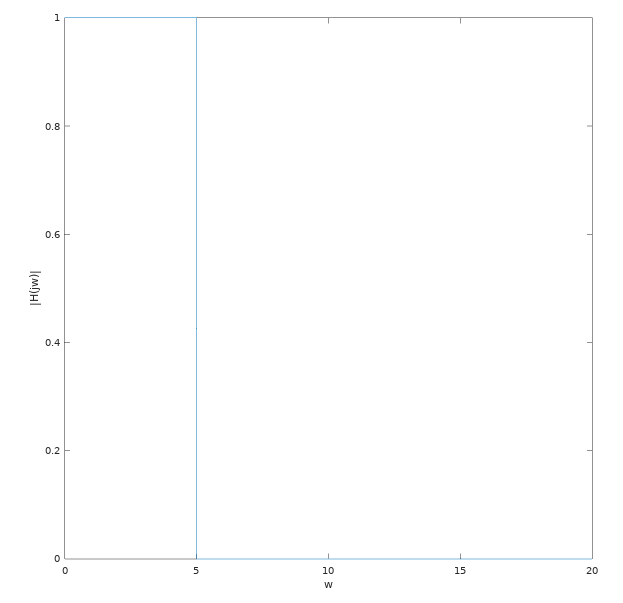
\includegraphics[width=0.5\textwidth]{images/Hjw.png}
     \caption{Módulo de $H(j\omega)$}
 \end{figure}

 Módulo da saída $|Y(j\omega)| = |H(j\omega)||X(j\omega)|$:

 \begin{figure}[H]
 \centering
 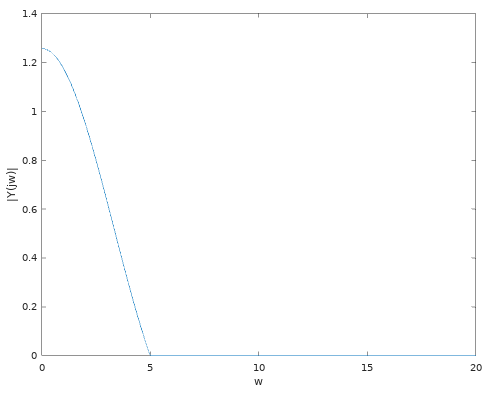
\includegraphics[width=0.5\textwidth]{images/Yjw.png}
     \caption{Módulo de $Y(j\omega)$}
 \end{figure}

\break\vfill

\item

    Gráfico com o módulo da resposta em frequência do filtro de Chebyshev ($|H_C(j\omega)|$) bem como o módulo da resposta do sinal $X(j\omega)$ ao passar pelo filtro:

 \begin{figure}[H]
 \centering
 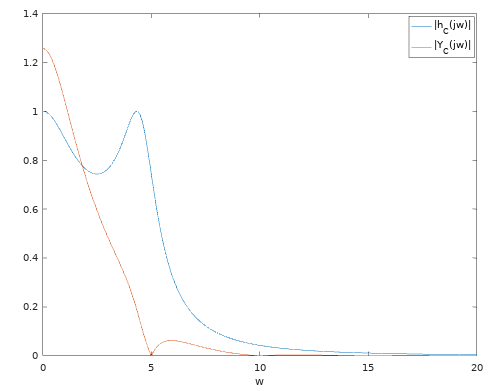
\includegraphics[width=0.5\textwidth]{images/hcyc.png}
     \caption{Módulo de $H_C(j\omega)$ e de $Y_C(j\omega)$}
 \end{figure}

\item

    Gráfico com o módulo da resposta em frequência do filtro de Butterworth ($|H_B(j\omega)|$) bem como o módulo da resposta do sinal $X(j\omega)$ ao passar pelo filtro:

 \begin{figure}[H]
 \centering
 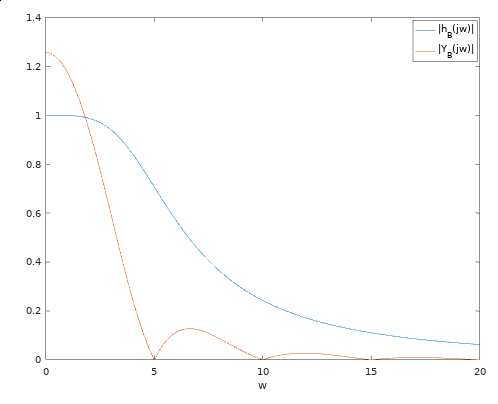
\includegraphics[width=0.5\textwidth]{images/hbyb.png}
     \caption{Módulo de $H_B(j\omega)$ e de $Y_B(j\omega)$}
 \end{figure}

\break\vfill

\item

    Gráficos respectivamente dos módulos de $H(j\omega)$ e dos módulos de $Y(j\omega)$:

 \begin{figure}[H]
 \centering
 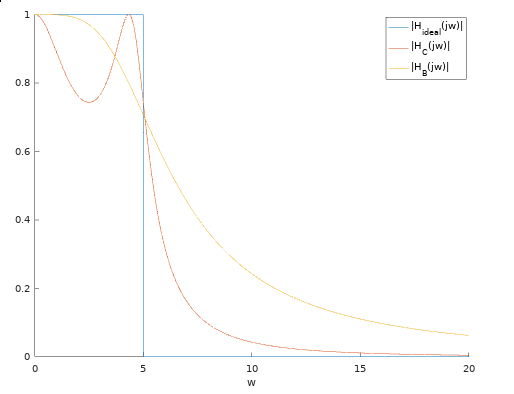
\includegraphics[width=0.5\textwidth]{images/hhchb.png}
     \caption{Módulo de $H(j\omega)$}
 \end{figure}

 \begin{figure}[H]
 \centering
 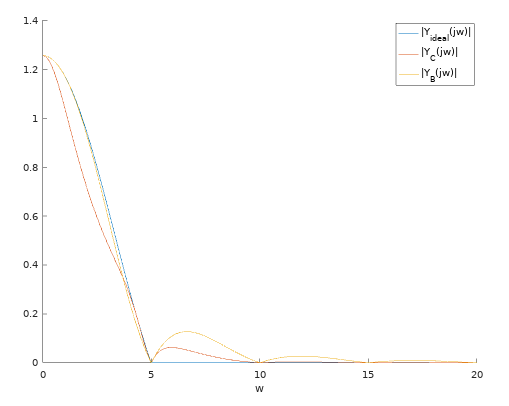
\includegraphics[width=0.5\textwidth]{images/yycyb.png}
     \caption{Módulo de $Y(j\omega)$}
 \end{figure}

 Como observado na primeira figura acima, o filtro de Chebyshev se comporta de maneira mais parecida à um filtro passa-baixa ideal para $\omega > \omega_C$, enquanto que o filtro de Butterworth se comporta de maneira mais parecida à um filtro passa-baixa ideal para $\omega < \omega_C$. Isso é perceptivel através da segunda figura em que $Y_B$ é praticamente a mesma curva que a saída do filtro ideal para frequências pequenas, enquanto que $Y_C$ apresenta menos deformações na curva (em relação à saída do filtro ideal) para $\omega > \omega_C$, mas apresenta mais deformação para frequências mais baixas ($\omega < \omega_C$). Mesmo assim é possível perceber que ambos se comportam como filtros passa-baixa (ganho elevado para frequências baixas e ganho próximo a zero para frequências altas) e isso se reflete em respostas que se assemelham muito com o sinal de entrada para $\omega < \omega_C$ e são muito próximos de zero para $\omega > \omega_C$.

\end{enumerate}
\end{document}
